\documentclass{article}
\usepackage{amsmath}

\title{Simple Linear Regression Analysis}
\author{PHILHOON OH}

\usepackage{Sweave}
\begin{document}
\Sconcordance{concordance:lab9.tex:lab9.Rnw:%
1 6 1 1 0 31 1 1 5 10 0 1 2 6 1 1 4 11 0 1 2 16 1}

\maketitle

\section{Abstract}
In this report, I will reproduce the main results displayed in section 3.1 \emph{Simple Linear Regression (chapter3)} of the book \emph{An introduction to Statistical Learning} descirbed below : 
\begin{itemize}
\item Figure 3.1 (page 62) Scatterplot with fitted regression line (the vertical distances of each point to the line are optional).  
\item Table 3.1 (page 68) Summary of regression coefficients.  
\item Table 3.2 (page 69) Quality indices RSE, R square, and F-statistic. efforts on demonstrating that reinforcement learning can be made peer-to-peer, autonomous, and cacheable.
\end{itemize}


\section{Introduction}
The goal of this homework is to reproduce the results of Explanatory Data Analysis on TV advertising budget and Sales and see if there is a assoication between them. If so, using linear regression we will see how they are correlated and how accurate model that can be used to predict sales based on the TV advertising budgets.


\section{Data}
Data set consists of the Sales(in thousand of units) of a certain products in 200 different markets, and the advertising budgets of 3 differnet media: TV, Radio, and Newspaper (4 variabales and 200 observations.) Since we are focusing on the TV and Sales, first we need to extract the data and applying the simple linear regression.


\section{Methodology}
I will apply a simple linear regression model to see the linear relationship between TV advertising budgets and the Sales:

$$\\Sales = \beta_{0} + \beta_{1}TV$$ 

To estimate the coefficients $\beta_{0}$ and $\beta_{1}$ we fit a regression model via the least squares criterion (Best Linear Prediction method).

\section{Results}
The regression coefficients are discribed below in a table:

\begin{table}[ht]
\centering
\begin{tabular}{rrrrr}
  \hline
 & Estimate & Std. Error & t value & Pr($>$$|$t$|$) \\ 
  \hline
(Intercept) & 7.0326 & 0.4578 & 15.3603 & 0.0000 \\ 
  tv & 0.0475 & 0.0027 & 17.6676 & 0.0000 \\ 
   \hline
\end{tabular}
\caption{Information about Regression Coefficients} 
\end{table}   
Under the null hyopthesis, p-value of intercept is significant to reject the null. The estimate of the   intercept is 7.03259 with sd of 0.45784

Under the null hyopthesis, p-value of slope is significant to reject the null. The estimate of the slope is 0.45784 with sd of 0.00269\\

Quality indices RSE, R square, and F-statistic are given in the table below: 

\begin{table}[ht]
\centering
\begin{tabular}{rlr}
  \hline
 & Quantity & Value \\ 
  \hline
1 & R2 & 0.6119 \\ 
  2 & RSE & 3.2587 \\ 
  3 & F-stat & 312.1450 \\ 
   \hline
\end{tabular}
\caption{Regression Quality Indices} 
\end{table}

R sqaure is the percent of variation that can be explained by the regression equation. It means that about 61.18751 precent of variations in sales can be explained by the regression equation.

Residual Standard Error refers the estimated standard error of residuals. It measures the distance between the data point and the regression equation. Here, RSE is 3.25866 on 198 degrees of freedom.

In simple linear regression, null hypothesis of F-test is 'slope equals to zero.' Here, F-statistics is 312.14499 which is significant to reject the null.


\begin{figure}[!htb]
  \begin{center}
    \caption{Scatterplot with fitted regression line}
    \centering
      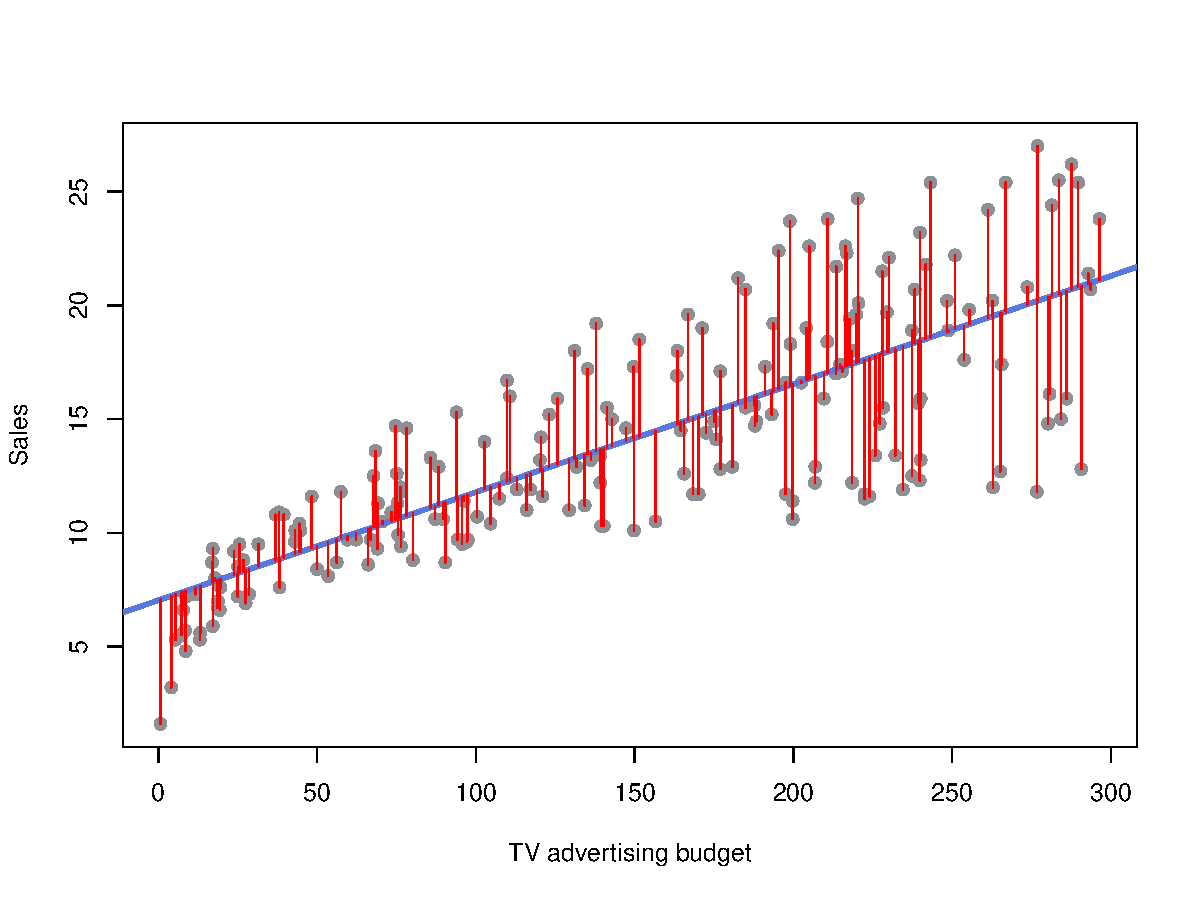
\includegraphics[width=4in]{scatterplot-tv-sales.pdf}
  \end{center}
\end{figure}


\section{Conclusions}
According to the Table 2, F-statistics indicates to reject the null hypothesis, $H_0 : \beta_{1} = 0$. Therefore, there is a linear relationship between `TV advertising budgets` and `Sales.` It is the same result when we test with the correlation coefficient presented in Table1. In the plot, it seems that there are slightly more variations at both ends. However, the data shows pretty good linear relationship between TV advertising and the Sales. 1000 standard unit increase in TV advertising, increases 47 standard units in sales. Thus, it is safe to conclude that there is a linear relationship between them. 


\end{document}
